\section{Appendix}

\subsection{Supplemental Experiments}
We present a simplified GridWorld example to illustrate the structure of tasks amenable to segmentation. 

\vspace{0.5em} \noindent \textbf{Motivating Experiments: } Before we discuss segmentation, the first hypothesis that we have to evaluate is whether IRL on its own can improve the convergence of RL. This hypothesis is not unreasonable since some problem have a naturally sparse reward function (e.g., 1 if a goal state is reached, 0 else where), and IRL would approximate this reward with a smoother quadratic function. So consider an 16 x 16 GridWorld with a start position in one corner and a goal in another corner (Figure \ref{concept:1}a). 
The agent can move left, right, up, and down, and with a 30\% probability the action results in a random motion.
We sampled 5 demonstrations with a value iteration supervisor and applied IRL with linear and quadratic rewards. These results are visualized in (Figure \ref{concept:1}b-c).
These plots illustrate how IRL can be used to shape a reward function, by changing the reward parametrization. Even though the underlying reward function is a sparse 1/0 reward,  MaxEnt fits a linear or a quadratic reward function, which is smoother. These smoother reward functions can help guide the agent to the goal.

\begin{figure}[ht]
\centering
 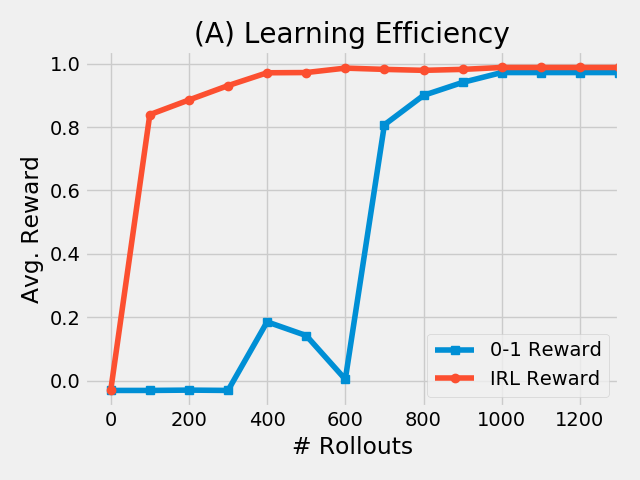
\includegraphics[width=0.48\columnwidth]{concept/1.png}
  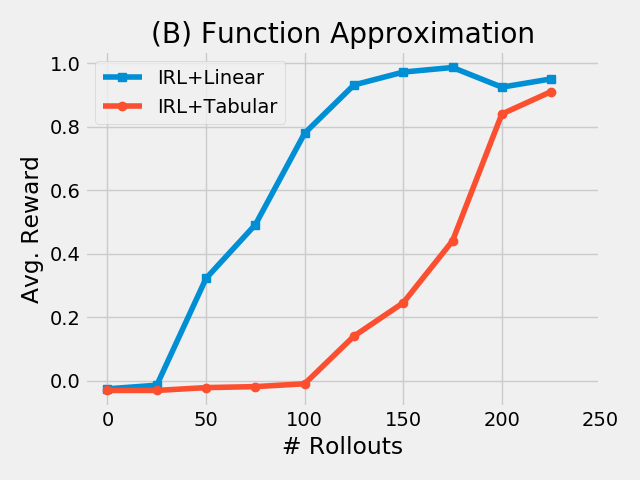
\includegraphics[width=0.48\columnwidth]{concept/2.png}
 \caption{(A) Tabular Q-Learning converges nearly 8x faster when the reward is quadratically shaped by IRL. (B) These benefits are even more pronounced when the Q function is approximated by a linear regression model. \label{concept:2}}
\end{figure}

\begin{figure}[ht]
\centering
 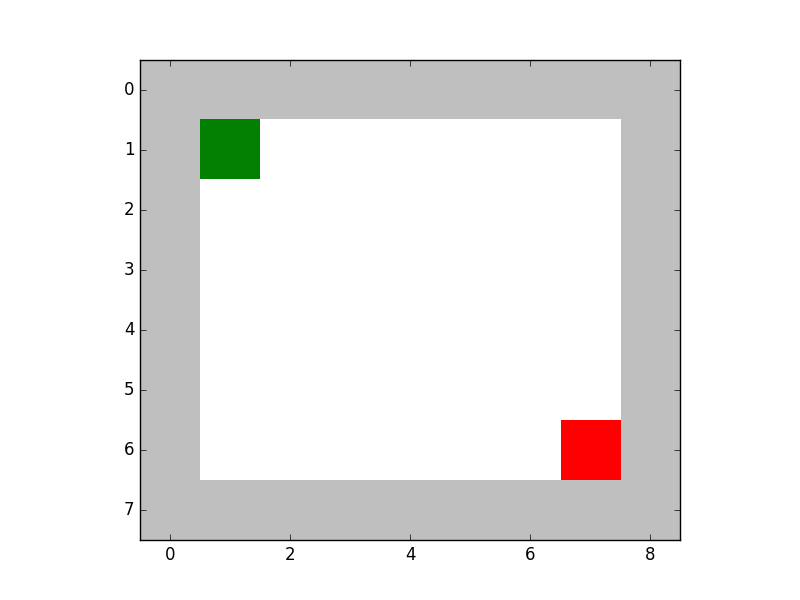
\includegraphics[width=0.32\columnwidth]{concept/swirl1-rewards.png}
  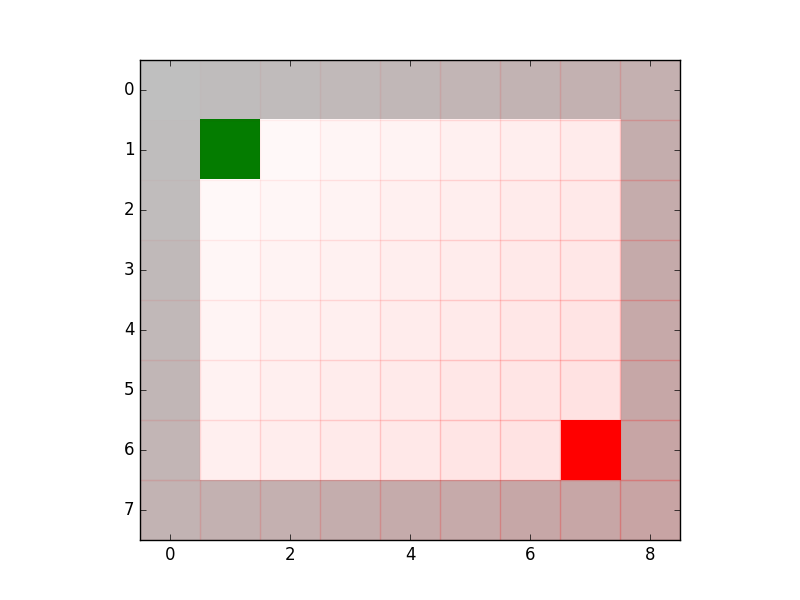
\includegraphics[width=0.32\columnwidth]{concept/swirl1-linear.png}
   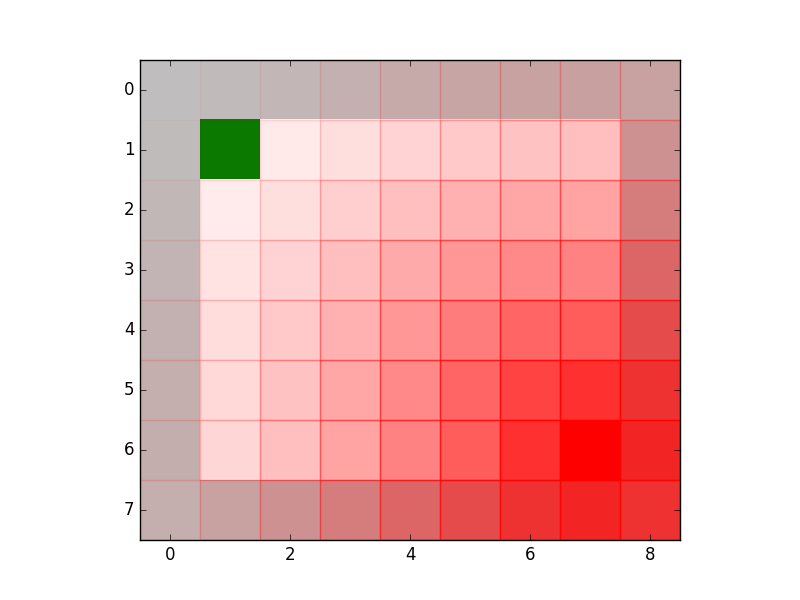
\includegraphics[width=0.32\columnwidth]{concept/swirl1-quadratic.png}
 \caption{This plot illustrates a conceptual GridWorld task. The green square denotes the starting position and the red denotes the target. The first plot shows the basic task, the second plot shows the reward learned with IRL from 5 demonstrations with a linear reward parametrization, and the second plot shows the reward learned with a quadratic parametrization. \label{concept:1}}
\end{figure}

If we were to compare the convergence of RL on the 1/0 reward and the quadratic reward, we find vastly different convergence properties.
We use a tabular Q-Learning agent with an $\epsilon$-greedy exploration policy ($\epsilon=0.1$).
Q-Learning on the quadratic reward converges in nearly 8x fewer steps than the 1/0 reward (Figure \ref{concept:2}a).
This is because the Q-Learning agent with the shaped reward function observes a reward earlier than the 0/1 agent, and thus, it is able to make progress towards the goal earlier in the learning process.
Combining function approximation with Q-Learning allows it to generalize to nearby unseen states.
The effects are even more pronounced since now once the agent observes the ``right direction'' to travel due to the shaped reward it is able to quickly make progress (Figure \ref{concept:2}b).
In the following experiments, we will use the term \textsf{IRL} to refer to the combined IRL+RL policy inference procedure.

\begin{figure}[t]
\centering
 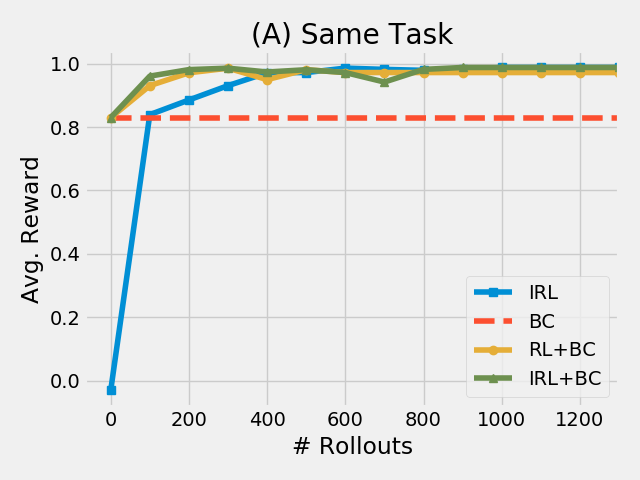
\includegraphics[width=0.48\columnwidth]{concept/3.png}
  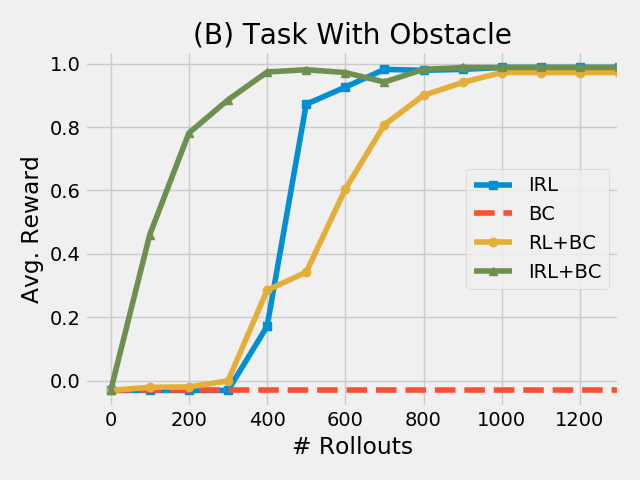
\includegraphics[width=0.48\columnwidth]{concept/4.png}
 \caption{(A) Given 5 expert demonstrations, Behavioral Cloning with a Random Forest classifier achieves a high reward on the same task. This can be used to initialize the Q-Learning agents. On the same task there is a marginal benefit to IRL. (B) We perturb the task after collecting 5 demonstrations by adding an obstacle blocking the shortest path, and find that the IRL agent is the most effective.  \label{concept:3}}
\end{figure}

One could hand-craft such reward functions, but one advantage of IRL is that it learns such functions from demonstration data. Admittedly, the previous comparison with RL is not completely fair. The RL algorithm with the 1/0 reward does not use the demonstration data. In principle, one could train a policy with Behavioral Cloning and use that to initialize the RL agent. Given the same 5 initial demonstrations, we train a random forest classifier.
When we apply this policy to the same task instance where the demonstrations were collected, the behavioral cloning policy does very well (Figure \ref{concept:3}a).
This can be used as an initialization to the Q-learning agent, which can further improve the policy.
On the same task instance, there is a marginal benefit to using IRL to shape the reward--as the behavioral cloning policy already gets the agent very close to the goal in most cases.

However, suppose that demonstration domain slightly differs from the execution domain. We simulate this by adding a 4x4 obstacle in the center of the GridWorld map.
Now, the learned behavioral cloning policy is not effective on the new domain (Figure \ref{concept:3}b).
However, the reward function learned with IRL transfers more robustly.
Furthermore, combining the IRL with a BC initialization improves performance over RL by 6x.
These results motivate us to consider how to use demonstrations to improve the convergence of RL.
In more complex tasks, a quadratic approximation of the reward may not suffice.
Hence, we consider how to segment the task into sub-tasks that can be approximated with a quadratic reward.


\begin{figure}[t]
\centering
 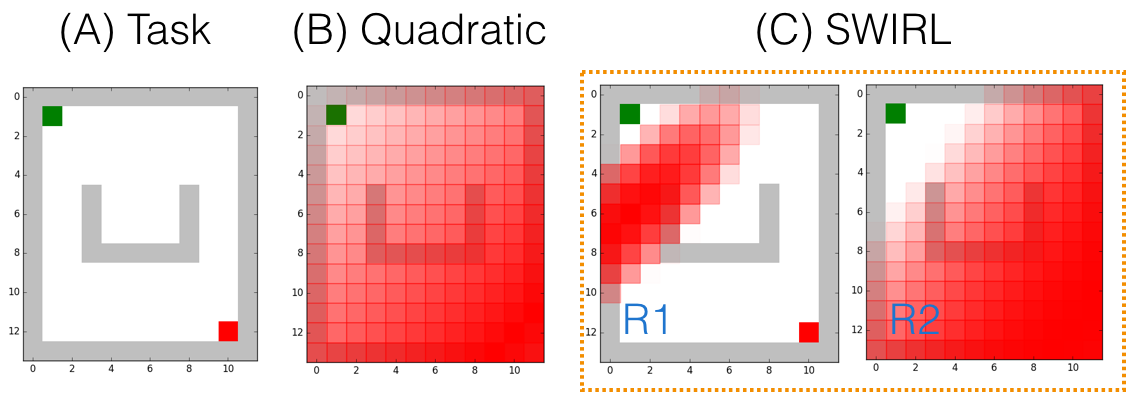
\includegraphics[width=\columnwidth]{concept/swirl-rewards.png}
 \caption{(A) A GridWorld domain with an obstacle, (B) Visualization of the reward function if we apply IRL to 5 demonstrations and fit a quadratic reward. The quadratic reward can encourage the agent to get ``stuck'' in the obstacle if it is too greedy, (C) Segmented quadratic reward function learned with \hirl. The function has two components first guiding the agent to the passage on the left, and then guiding to the goal.  \label{concept:4}}
\end{figure}

\begin{figure}[t]
\centering
 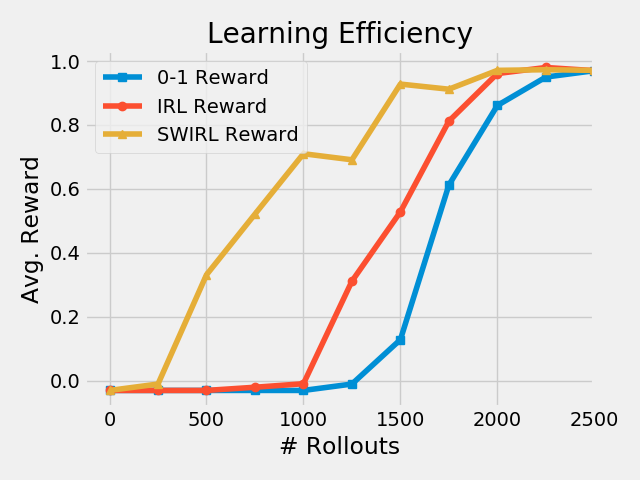
\includegraphics[width=0.6\columnwidth]{concept/2-1.png}
 \caption{\hirl converges faster than a single quadratic reward or the 1-0 reward. \label{concept:5}}
\end{figure}


\vspace{0.5em} \noindent \textbf{Hypothesis 0. IRL Can Benefit From Segmentation: } Now, we make the domain above slightly more complicated. We add an obstacle in such a way that the straight-line path is no longer optimal (Figure \ref{concept:4}a). As before, we sample 5 demonstrations from a value iteration supervisor.
Qualitatively, the quadratic reward learned from IRL is misleading as it can guide an overly greedy agent into the obstacle(Figure \ref{concept:4}b). 
\hirl learns a two-segment reward, where first it guides the agent to a point in the left passage and then a reward around the goal (Figure \ref{concept:4}c).
The number of segments was determined by a Dirichlet process prior as described in the text.

To evaluate \hirl quantitatively, we use a tabular Q-learning agent to learn a policy using these rewards.
To control for initialization effects, the agents were initialized randomly (unlike the previous experiment) and used an $\epsilon=0.1$ exploration policy.
This results in a significant improvement in convergence as seen in Figure \label{concept:5}.

\begin{figure}[t]
\centering
 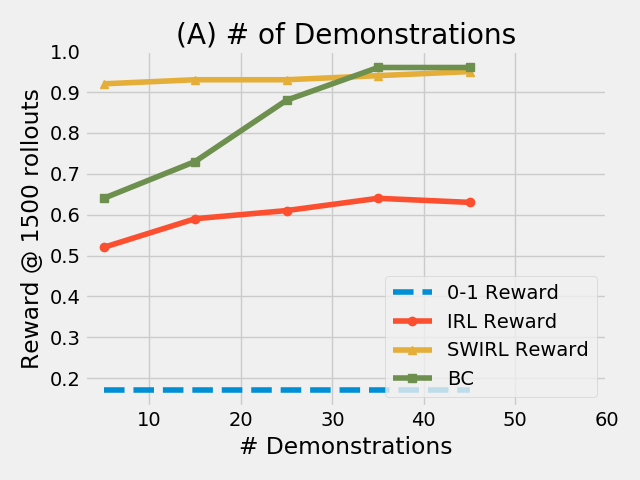
\includegraphics[width=0.48\columnwidth]{concept/3-1.png}
  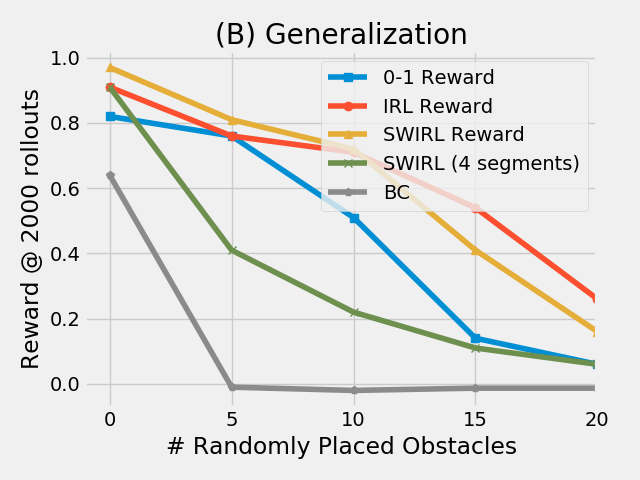
\includegraphics[width=0.48\columnwidth]{concept/3-2.png}
 \caption{(A) We measure the sensitivity to the number of initial demonstrations, (B) We perturb the execution environment by adding random obstacles. \label{concept:6}}
\end{figure}

\vspace{0.5em} \noindent \textbf{Parameter Sensitivity: } Finally, we use the previous GridWorld environment to illustrate the sensitivity to different parameters. In Figure \ref{concept:6}a, we vary the number of initial demonstrations provided to IRL and Behavioral Cloning and measure the performance after 1500 rollouts.
IRL is not as sensitive to the number of demonstrations as BC.
This is because the reward function that IRL is estimating is much simpler than policy function.
Next, we evaluate each of the algorithms on their ability to generalize to different task instances.
We perturb the execution environment by randomly adding single grid point obstacles.
We average the results over 50 such random perturbations (Figure \ref{concept:6}b).

Not surprisingly, we find that IRL is the most robust.
\hirl is relatively robust but is slightly worse than IRL for a large number of random obstacles.
We wanted to understand why \hirl was less robust than standard IRL, so we manually set the number of segments in \hirl to $4$.
The performance of \hirl with 4 segments is much worse.
This is because obstacles can ``invalidate'' segments.
This suggests an interesting tradeoff where more segments can serve to more precisely guide the agent towards the goal, but less segments lead to improved generalization.